\documentclass{standalone}
\usepackage{graphicx}	
\usepackage{amssymb, amsmath, amsthm}
\usepackage{color}

\usepackage{tikz}
\usetikzlibrary{intersections, backgrounds, math, arrows.meta}

\definecolor{light}{RGB}{220, 188, 188}
\definecolor{mid}{RGB}{185, 124, 124}
\definecolor{dark}{RGB}{143, 39, 39}
\definecolor{highlight}{RGB}{180, 31, 180}
\definecolor{darkteal}{RGB}{29, 79, 79}
\definecolor{darkolive}{RGB}{97, 123, 45}
\definecolor{gray10}{gray}{0.1}
\definecolor{gray20}{gray}{0.2}
\definecolor{gray30}{gray}{0.3}
\definecolor{gray40}{gray}{0.4}
\definecolor{gray60}{gray}{0.6}
\definecolor{gray70}{gray}{0.7}
\definecolor{gray80}{gray}{0.8}
\definecolor{gray90}{gray}{0.9}
\definecolor{gray95}{gray}{0.95}

\begin{document}

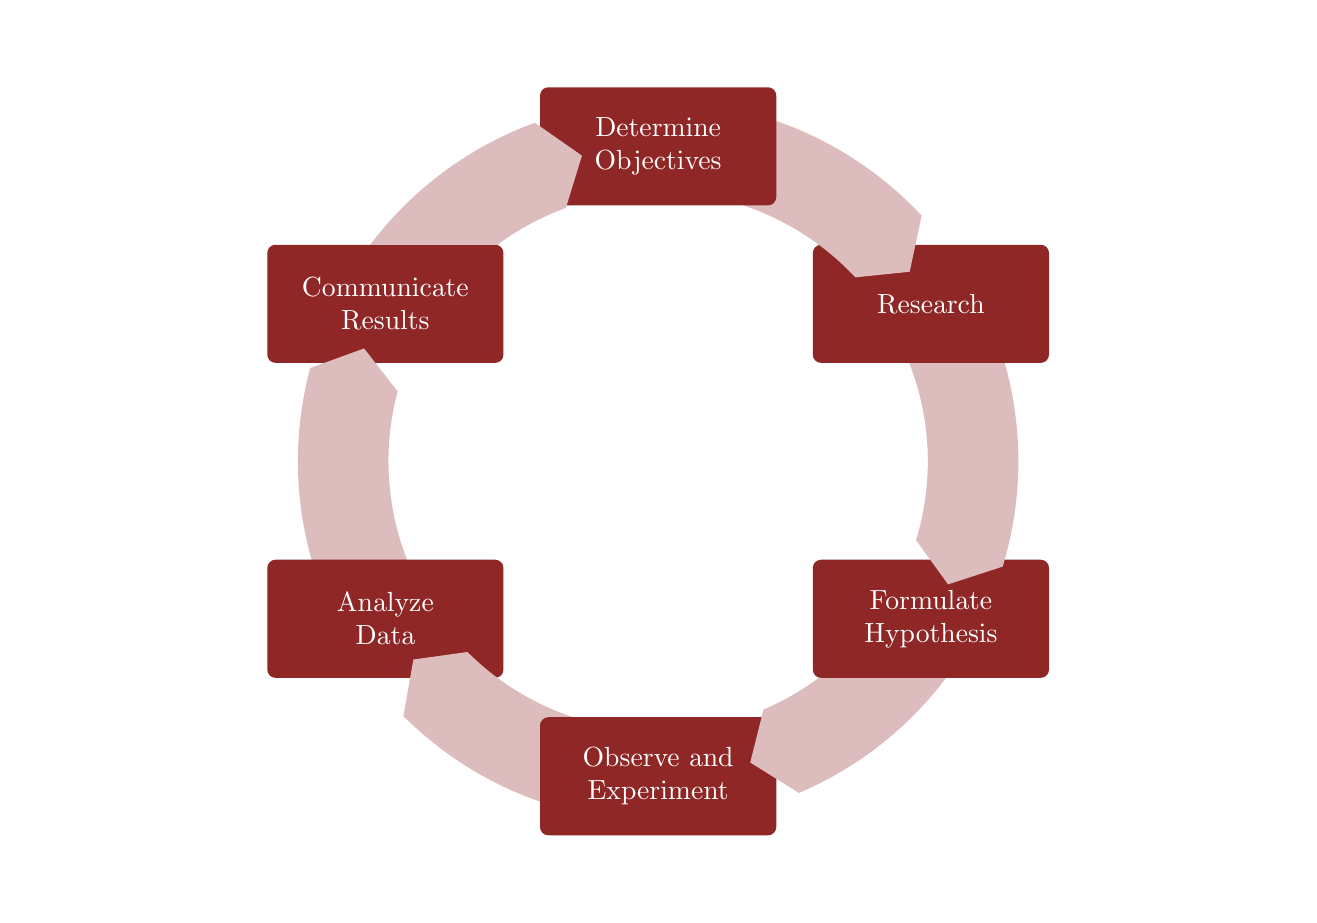
\begin{tikzpicture}[scale=1.0]
  
  \draw[white] (-8, -5.5) rectangle (8, 5.5);

  \pgfmathsetmacro{\dx}{3}
  \pgfmathsetmacro{\dy}{1.5}
  \pgfmathsetmacro{\r}{4}
  \pgfmathsetmacro{\dr}{0.575}
  \pgfmathsetmacro{\dt}{-6}

  \fill[rounded corners=3, fill=dark, text=white] 
    ({\r * cos(-210) - 0.5 * \dx}, {\r * sin(-210) - 0.5 * \dy}) rectangle +(\dx, \dy)
  node [midway, align=center] {Communicate\\Results};

  \pgfmathsetmacro{\thetai}{210}
  \pgfmathsetmacro{\thetaf}{165}

  \fill[light] (\thetai:{\r + \dr}) arc(\thetai:\thetaf:{\r + \dr}) -- 
               ({\r * cos(\thetaf + \dt)}, {\r * sin(\thetaf + \dt)}) --
               (\thetaf:{\r - \dr}) arc(\thetaf:\thetai:{\r - \dr})  -- cycle;

  \fill[rounded corners=3, fill=dark, text=white] 
    ({\r * cos(-150) - 0.5 * \dx}, {\r * sin(-150) - 0.5 * \dy}) rectangle +(\dx, \dy)
  node [midway, align=center] {Analyze\\Data};

  \pgfmathsetmacro{\thetai}{-90}
  \pgfmathsetmacro{\thetaf}{-135}

  \fill[light] (\thetai:{\r + \dr}) arc(\thetai:\thetaf:{\r + \dr}) -- 
               ({\r * cos(\thetaf + \dt)}, {\r * sin(\thetaf + \dt)}) --
               (\thetaf:{\r - \dr}) arc(\thetaf:\thetai:{\r - \dr})  -- cycle;
  
  \fill[rounded corners=3, fill=dark, text=white] 
    ({\r * cos(-90) - 0.5 * \dx}, {\r * sin(-90) - 0.5 * \dy}) rectangle +(\dx, \dy) 
  node [midway, align=center] {Observe and\\Experiment};

  \pgfmathsetmacro{\thetai}{-30}
  \pgfmathsetmacro{\thetaf}{-67}

  \fill[light] (\thetai:{\r + \dr}) arc(\thetai:\thetaf:{\r + \dr}) -- 
               ({\r * cos(\thetaf + \dt)}, {\r * sin(\thetaf + \dt)}) --
               (\thetaf:{\r - \dr}) arc(\thetaf:\thetai:{\r - \dr})  -- cycle;

  \fill[rounded corners=3, fill=dark, text=white] 
    ({\r * cos(-30) - 0.5 * \dx}, {\r * sin(-30) - 0.5 * \dy}) rectangle +(\dx, \dy) 
  node [midway, align=center] {Formulate\\Hypothesis};

  \pgfmathsetmacro{\thetai}{30}
  \pgfmathsetmacro{\thetaf}{-17}

  \fill[light] (\thetai:{\r + \dr}) arc(\thetai:\thetaf:{\r + \dr}) -- 
               ({\r * cos(\thetaf + \dt)}, {\r * sin(\thetaf + \dt)}) --
               (\thetaf:{\r - \dr}) arc(\thetaf:\thetai:{\r - \dr})  -- cycle;

  \fill[rounded corners=3, fill=dark, text=white] 
    ({\r * cos(30) - 0.5 * \dx}, {\r * sin(30) - 0.5 * \dy}) rectangle +(\dx, \dy)
  node [midway, align=center] {Research};

  \pgfmathsetmacro{\thetai}{90}
  \pgfmathsetmacro{\thetaf}{43}

  \fill[light] (\thetai:{\r + \dr}) arc(\thetai:\thetaf:{\r + \dr}) -- 
               ({\r * cos(\thetaf + \dt)}, {\r * sin(\thetaf + \dt)}) --
               (\thetaf:{\r - \dr}) arc(\thetaf:\thetai:{\r - \dr})  -- cycle;

  \fill[rounded corners=3, fill=dark, text=white] 
    ({\r * cos(90) - 0.5 * \dx}, {\r * sin(90) - 0.5 * \dy}) rectangle +(\dx, \dy) 
  node [midway, align=center] {Determine\\Objectives};

  \pgfmathsetmacro{\thetai}{150}
  \pgfmathsetmacro{\thetaf}{110}

  \begin{scope}
    \clip (-\r, {\r * sin(-210) + 0.5 * \dy}) rectangle +(2 * \r, 2);
    \fill[light] (\thetai:{\r + \dr}) arc(\thetai:\thetaf:{\r + \dr}) -- 
                 ({\r * cos(\thetaf + \dt)}, {\r * sin(\thetaf + \dt)}) --
                 (\thetaf:{\r - \dr}) arc(\thetaf:\thetai:{\r - \dr})  -- cycle;
  \end{scope}
  
\end{tikzpicture}

\end{document}  